\documentclass[10pt, a4paper]{article}
\usepackage[utf8]{inputenc}
\usepackage[T1]{fontenc,url}
\usepackage{multicol}
\usepackage{multirow}
\usepackage{parskip}
\usepackage{lmodern}
\usepackage{microtype}
\usepackage{verbatim}
\usepackage{amsmath, amssymb}
\usepackage{tikz}
\usepackage{physics}
\usepackage{mathtools}
\usepackage{algorithm}
\usepackage{algpseudocode}
\usepackage{listings}
\usepackage{enumerate}
\usepackage{graphicx}
\usepackage{float}
\usepackage{hyperref}
\usepackage{tabularx}
\usepackage{siunitx}
\usepackage{fancyvrb}
%\usepackage{natbib}
%\bibliographystyle{dinat}
\usepackage[makeroom]{cancel}
\usepackage[margin=2.0cm]{geometry}
\usepackage{pdfpages}
\usepackage[margin=10pt, textfont={small, it}, labelfont={bf}, labelsep=endash]{caption}
\renewcommand{\baselinestretch}{1}
\renewcommand{\exp}{e^}
\renewcommand{\b}{\boldsymbol}
\newcommand{\h}{\hat}
\newcommand{\m}{\mathbb}
\newcommand{\half}{\frac{1}{2}}
\renewcommand{\exp}{e^}
\renewcommand{\bar}{\overline}
\setlength\parindent{0pt}


\begin{document}
\title{AST5220\\ Milestone I -- Background Cosmology}
\author{
    \begin{tabular}{r l}
        Jonas Gahr Sturtzel Lunde & (\texttt{jonassl})
    \end{tabular}}
% \date{}    % if commented out, the date is set to the current date

\maketitle
Code found at \url{https://github.com/asdfbat/AST5220/tree/master/Project}
\vspace{0.7cm}

\section{Theory}
\subsection{Components of the universe}
We consider a flat, expanding universe, governed by the $\Lambda \text{CDM}$ model. Our universe contains some densities of baryonic matter ($\rho_b$), cold dark matter ($\rho_{CDM}$), radiation ($\rho_r$), and dark energy ($\rho_\Lambda$). Let $\Omega_i = \dfrac{\rho_i}{\rho_c}$ be the \textit{relative densities} of each component. Here, $\rho_c$ is the \textit{critical density}, being the total density which would make the universe entirely flat. We will consider a flat universe (as ours is believed to be), from which it follows that
\begin{equation}\label{eqn:sum1}
    \sum_i \rho_i = \rho_c \quad \Rightarrow \quad \sum_i \Omega_i = 1
\end{equation}
We also define $\rho_{i,o}$ and $\Omega_{i,o}$ to represents the critical and relative densities today.

It can be shown \cite{ModernCosmology2003} that the density components evolve with time as $\rho_i(a) = \rho_{i,0}a^{-3(1+w_i)}$ where $w_i$ is some constant for each density component. For our four components, the densities evolve as
\begin{align*}
    \rho_b &= \rho_{b,0} a^{-3} \\
    \rho_\text{CDM} &= \rho_{\text{CDM},0} a^{-3} \\
    \rho_r &= \rho_{r,0} a^{-4} \\
    \rho_\Lambda &= \rho_{\Lambda,0}
\end{align*}
where $a$ is the \textit{scale factor} of the universe, describing its relative size to today. Today's value is defined to be $a_0 = 1$.

We wish to avoid the absolute densities where possible, and work directly with the relative densities and the scale factor. The relative densities can be rewritten to exclude $\rho_i$ the following way:
\begin{align*}
    \Omega_{i} = \frac{\rho_i}{\rho_c} = \frac{\rho_{i,0}a^{-3(1+w_i)}}{\rho_c} = \frac{\rho_{c,0}\Omega_{i,0}a^{-3(1+w_i)}}{\rho_c}
\end{align*}

The critical density can be shown \cite{callin2006} to be $\rho_c = \frac{3H^2}{8\pi G}$, which gives $\rho_{c,0} = \frac{3H_0^2}{8\pi G}$, such that we can write
\begin{align}\label{eqn:Omegas}
    \Omega_{i} = \qty(\frac{H_0}{H})^2\Omega_{i,0}a^{-3(1+w_i)}
\end{align}


\subsection{The Friedmann equation}
The evolution of the scale factor is governed by the (first) Friedmann equation, which for the universe described above reads \cite{callin2006}
\begin{equation}
    H(a) = \frac{\dot{a}}{a} = H_0\sqrt{\Omega_{b,0} a^{-3} + \Omega_\text{{CDM},0}a^{-3} + \Omega_{r,0}a^{-4} + \Omega_{\Lambda,0}}
\end{equation}

Since the universe takes on scales of many different orders of magnitude, the linear scale factor $a$ is not always well suited for analysis of large time spans. We introduce time(and scale) quantity
\begin{equation}
    x = \log{a} \quad \Rightarrow \quad a = \exp{x}
\end{equation}
The Friedmann equation now reads
\begin{equation} \label{eqn:Friedmann}
    H(x) = H_0\sqrt{\Omega_{b,0} e^{-3x} + \Omega_\text{{CDM},0}e^{-3x} + \Omega_{r,0}e^{-4x} + \Omega_{\Lambda,0}}
\end{equation}

We also introduce the scaled Hubble parameter $\mathcal{H} = aH = \dot{a}$.


\subsection{Conformal time}
As well as $a$, $x$, and $t$ for measuring time in the universe, we will introduce the conformal time $\eta$. $\eta$ has units of length, and represents the size of the event horizon at any given time. In other words, $\eta$ is the distance traversed by undisturbed light since the Big Bang. Conformal time is more commonly used with units of time, which follows from dividing our quantity by $c$, thereby having the interpretation of the time it would take a photon to traverse the universe at that given time (given that the expansion "froze" for the duration of the photons travel).

The conformal time, in units of length, takes on the form
\begin{equation}
    \eta = \int_0^t \frac{c}{a(t)} \dd{t}
\end{equation}

Or, on differential equation form
\begin{equation}
    \dv{\eta}{t} = \frac{c}{a}
\end{equation}

This can be written as a differential equation with regards to $a$.
\begin{equation*}
    \dv{\eta}{a}\dv{a}{t} = \dv{\eta}{a}\frac{1}{\mathcal{H}} = \frac{c}{a}
\end{equation*}

Resulting in the ODE
\begin{align}\label{eqn:eta}
    \dv{\eta}{a} = \frac{c}{a\mathcal{H}}
\end{align}

This, again, can be rewritten as a function of $x = \log(a)$ as
\begin{align*}
    \dv{\eta}{a} = \dv{\eta}{x}\dv{x}{a} = \dv{\eta}{x}\frac{1}{a}
\end{align*}

which, inserting into \ref{eqn:eta} gives us the ODE
\begin{align}\label{eqn:etaODE}
    \dv{\eta}{x} = \frac{c}{\mathcal{H}}
\end{align}


\subsection{Analytical solution to conformal time}\label{sec:conf}
The conformal time integral is not analytically solvable for the complete Hubble parameter, but analytical solutions exist in each of the dominant regimes (radiation, matter, DE). In the radiation dominated regime, $\eta$ takes the form
\begin{align}
    \eta_r = \frac{c}{aH_r(a)},  \quad  H_r(a) = H_0\sqrt{\Omega_{r,0} a^{4}}.
\end{align}

In the matter dominated regime, $\eta$ takes the form
\begin{align}
    \eta_m = \eta(a_*) + 2c\qty[\frac{1}{aH_m(a)} - \frac{a_*^{1/2}}{a^{3/2}}], \quad H_m = H_0\sqrt{(\Omega_{b,0} + \Omega_{CDM,0}) a^3}.
\end{align}
where $a_*$ is some point where $\Omega_m \approx 1$.

In the DE dominated regime, $\eta$ takes the form
\begin{align}
    \eta_\Lambda = \eta(a_\Lambda) + \frac{c}{H_\Lambda(a)}\qty[\frac{1}{a_\Lambda} - \frac{1}{a}], \quad H_\Lambda(a) = \sqrt{\Omega_{\Lambda,0}}.
\end{align}
where $a_\Lambda$ is some point where $\Omega_\Lambda \approx 1$. The two latter equations require known values of $\eta$ at certain points, preferably deep within their own dominant regime. If only these analytical approximations are available, an extrapolated value of $\eta$ from the previous era would have to be used.

One possible enhancement of these expressions is to replace the final approximations of the Hubble parameters with the real deal. Even though the approximations are required to carry out the integral, we can insert the full Hubble parameter in place of the approximations in the final expression - $H_m = H_r = H_{\Lambda} = H$.


\section{Method and implementation}
\subsection{Code Overview}
The code for reproducing our results can be found at \url{https://github.com/asdfbat/AST5220/tree/master/Project}. The C++ programs solving all equations are found in the directory named \texttt{src}, where a \texttt{Makefile} runs all code. The central code for this project can be found in the \textit{BackgroundCosmology} class in the file \texttt{src/BackgroundCosmology.cpp}. The class relies heavily on an implementation of GSL's ODESolver, found in the file \texttt{src/ODESolver.cpp}, and an implementation of GSL's spline interpolator, found in \texttt{src/spline.cpp}.

Code for plotting all relevant results are found in \texttt{Python/m1\_plotting.py}.


\subsection{Density parameters and the Friedmann equation}
We find the scaled Hubble parameter $\mathcal{H}$ explicitly from the Friedmann equation \ref{eqn:Friedmann} for $x \in [-27.6, 4.6]$, using density values roughly corresponding to the best estimates of the $\Lambda$CDM model, found in \cite{callin2006}. More updated values can be found in \cite{Planck2015}, yet we choose the values from the former, for easier comparability. These are
\begin{align*}
    \Omega_{b,0} &= 0.046 \\
    \Omega_{CDM,0} &= 0.224
\end{align*}
while $\Omega_{r,0}$ is directly calculated from today's observed temperature of the CMB, at $T_{CMB,0} = \SI{2.725}{K}$, as
\begin{align*}
    \Omega_{r,0} = \frac{\pi^2}{15}\frac{\qty(k_bT_{CMB,0})^4}{\hbar^3c^5}\frac{8\pi G}{3H_0^2} = 5.043 \times 10^{-5}.
\end{align*}
Equation \ref{eqn:sum1} constrains $\Omega_\Lambda$ to
\begin{align*}
    \Omega_{\Lambda,0} &= 1 - \qty(\Omega_R + \Omega_{CDM} + \Omega_m) = 0.72995
\end{align*}
Using the Hubble parameter, we calculate the relative densities of all components from equation \ref{eqn:Omegas}.


\subsection{Conformal time}
Equation \ref{eqn:etaODE} is solved in the interval $x \in [-27.6, 4.6]$, using an implementation of GSL's ODESolver class. As initial condition, we assume $\eta(x_0 = -27.6) = 0$, which corresponds to assuming that the size of the particle horizon is zero at $a=e^{-27.6} = 10^{-12}$. Since our results focus on the region of $x \in [-15, 4]$, this should be a fine approximation.

In addition, we compare our numerical results to the analytical results described in section \ref{sec:conf}. We find $\eta(a_*)$ and $\eta(a_\Lambda)$ using both a purely analytical solution, extrapolating the previous solution, and "cheating", by inserting more correct numerical values. For both cases, we look at the behavior of the solutions using both the local approximations of the Hubble parameter ($H_m$, $H_r$...), and setting them equal to the full Hubble parameter $H_i = H(x)$.


\section{Results}
\subsection{Hubble parameters and conformal time}
Figure \ref{fig:H} shows the evolution of conformal time and the Hubble parameter over time. In the two bottom plots, the Hubble parameter shows three linear regimes, which corresponds to exponential dependence on $x$, and power-law dependence on $z$ and $a$. The three linear regimes are split by the matter-radiation equality, and the radiation-dark energy equality, both indicated in the plots. In the radiation dominated regime, $H \propto a^2$, during the matter dominated regime, $H \propto a^{1.5}$, and in the dark energy dominated regime, $H$ is constant.

The scaled Hubble parameter also shows three regimes of exponential dependence on $x$, although instead of leveling out, the DE regime shows it increasing. Since $\mathcal{H} = \dot{a}$, this regime has the universes expansion accelerating, while the radiation and matter dominated regimes have the expansion slowing down.

\subsection{Relative densities}
Figure \ref{fig:Omegas} shows the distribution of relative densities over time. We observe that the very early universe is completely radiation dominated, which gradually evolves into matter domination, the turnover point being at $x\approx-8.6$, or $z\approx 5350$. At $x\approx-3$, the universe energy content comes almost exclusively from baryons and CDM. This quickly transitions into the dark energy domination, at $x\approx -0.32$, or $z\approx 0.39$, which is the era we're in today. We also observe that the total relative density sums perfectly to 1 at all times.


\begin{figure}[H]
    \centering
    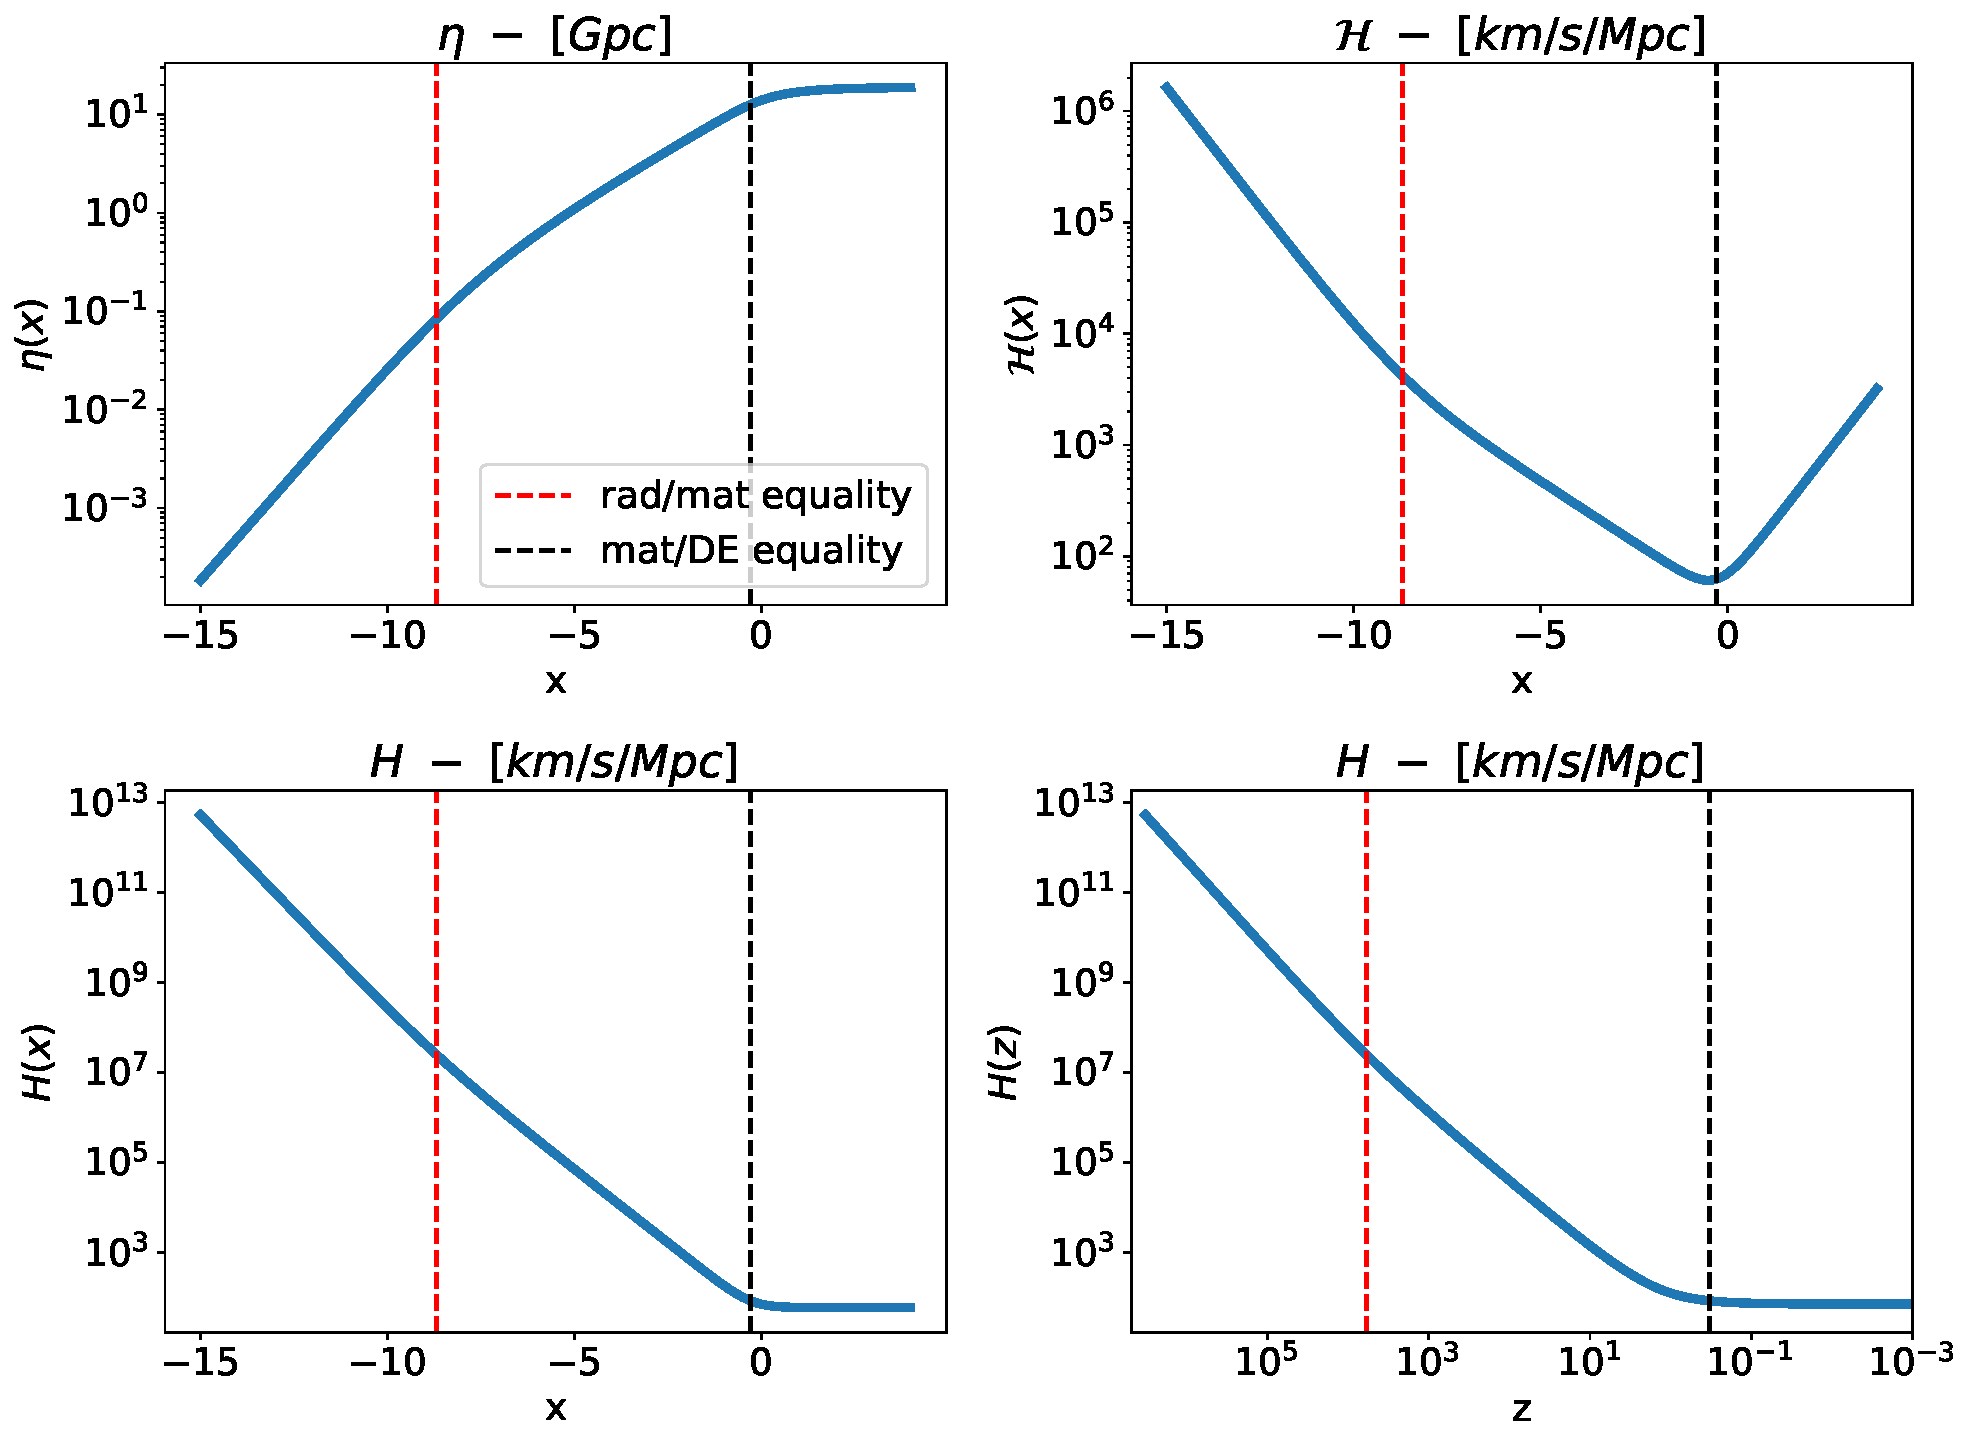
\includegraphics[scale=0.5]{../m1_figs/H.pdf}
    \caption{Plots showing the conformal time (top-right), the scaled Hubble parameter (top-right), and the Hubble parameter (bottom-left) as function of $x=\log{a}$. The bottom-right panel shows the Hubble parameter as function of redshift $z$. All plots show the matter-radiation equality as a striped red line, and the matter-dark energy equality as a striped black line.}
    \label{fig:H}
\end{figure}


\begin{figure}[H]
    \centering
    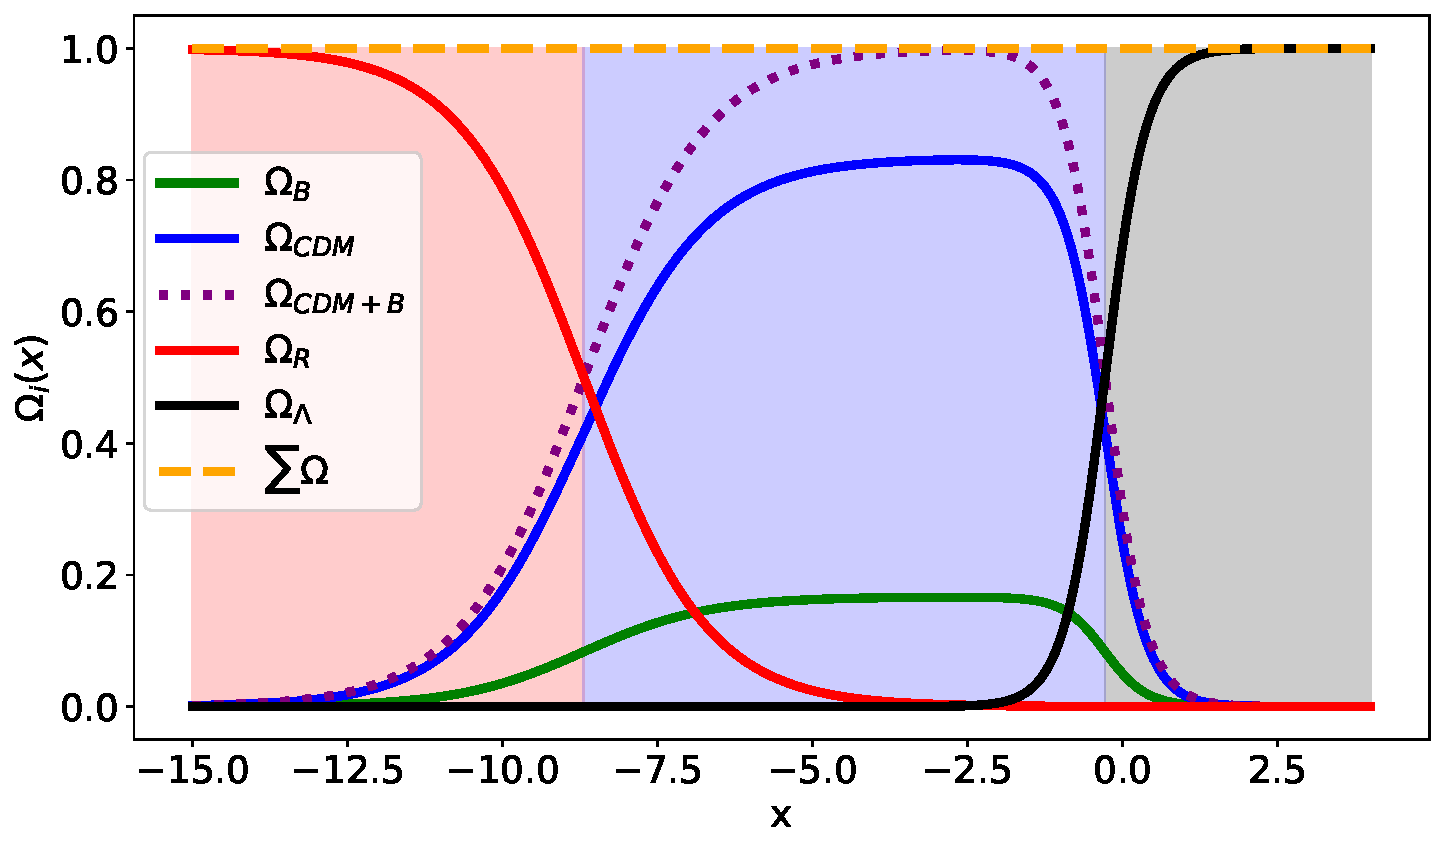
\includegraphics[scale=0.5]{../m1_figs/Omegas.pdf}
    \caption{Plot showing the relative density distribution of components as function of $x=\log{a}$. Radiation, matter, and dark energy dominated eras are highlighted in their respective colors.}
    \label{fig:Omegas}
\end{figure}

\subsection{Analytical solution of $\eta$}
Figure \ref{fig:Eta} shows the analyical solutions of $\eta(x)$ in the three regimes. Both plots anchor the value of $\eta$ at the maximum relative densities of each era, using numerical values. In other words, these plots are not entirely analytical, but show only the behavior of the analytical solutions when anchored to an exact value. On the left, we see the solutions when employing the local approximations of $H$, while the right plot employs the reinsertion of the entire Hubble parameter into the solution. Both approximations agree well when deep inside their own regime, but diverge quickly towards the edges. The behavior of the full-Hubble solution is obviously more complex, as it contains additional terms of x. Interestingly, the two solutions systematically diverge in opposite directions for all three regimes. For instance, for the local Hubble solutions (left) the extrapolated radiation dominated solution undershoots heavily into the matter dominated era, and overshoots heavily into the DE dominated era. This behavior is reversed for the full Hubble solution.

Figure \ref{fig:Eta2} shows the entire analytical approximation of $\eta(x)$, using extrapolated values from previous regimes. This would be our best approximations of $\eta$ if no numerical solution was available. The solution for both the re-inserted full Hubble parameter, and the local Hubble parameter are shown. We see that the approximations are comparably good. As in figure \ref{fig:Eta}, they over- and undershoot in exactly opposite ways.

\begin{figure}[H]
    \centering
    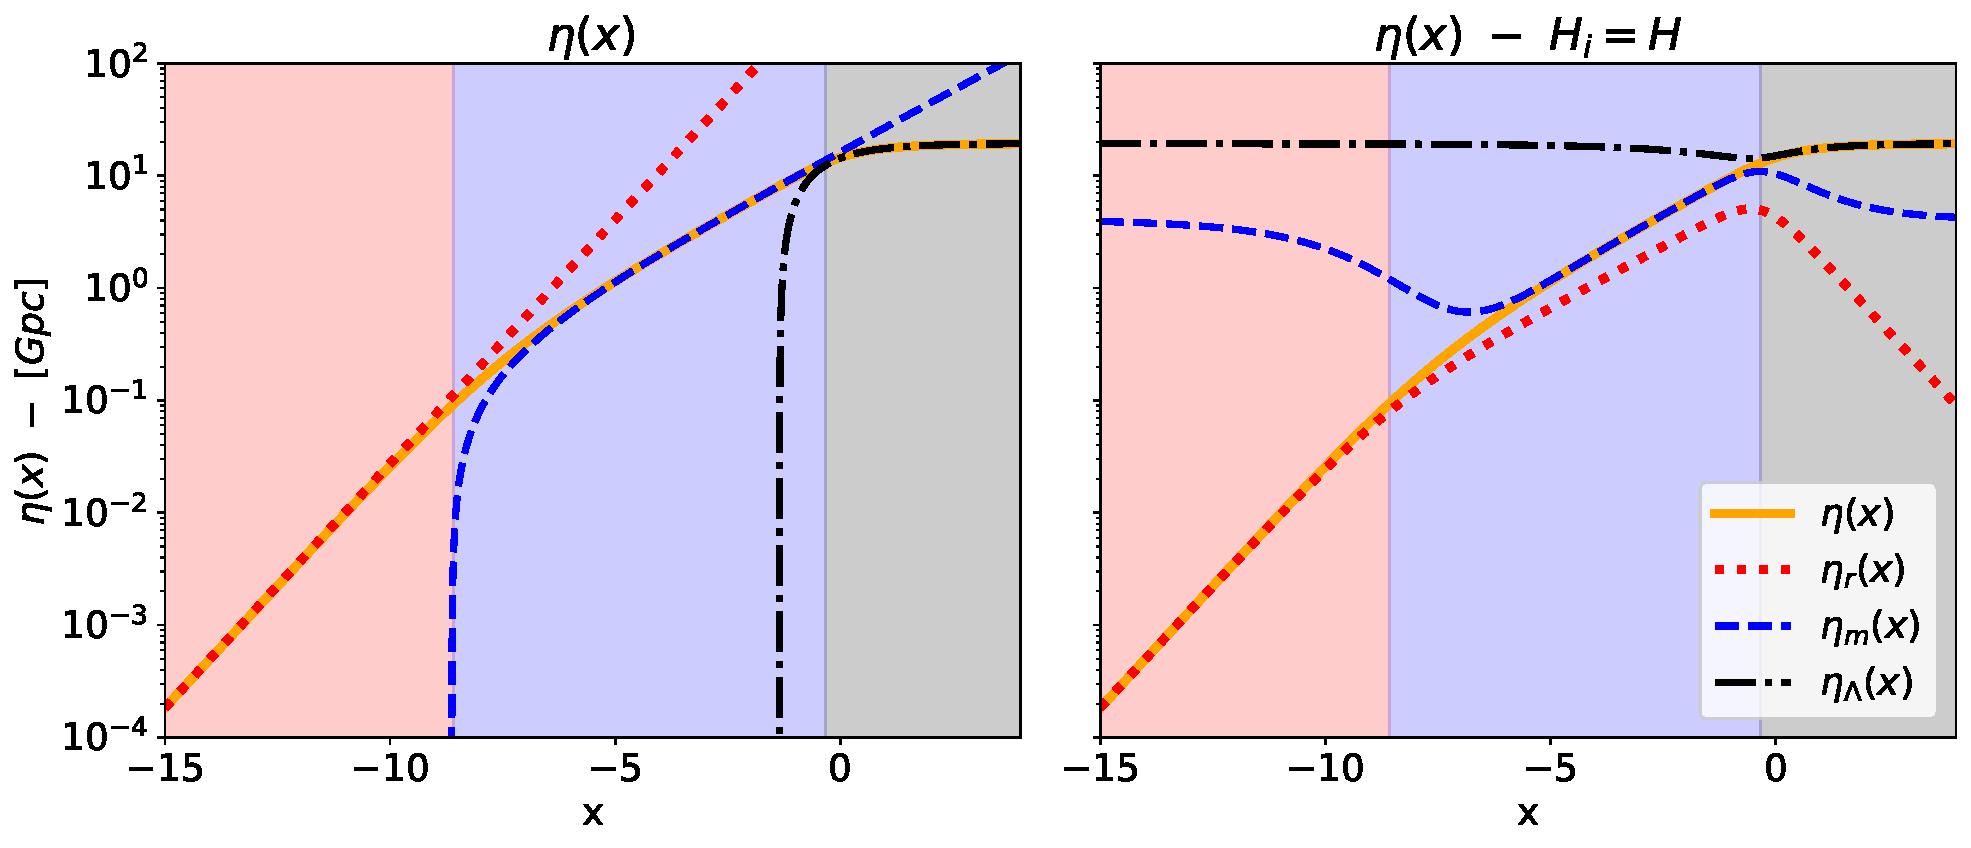
\includegraphics[scale=0.5]{../m1_figs/Eta.pdf}
    \caption{Plot showing the three analytical approximations of $\eta(x)$ in the three regimes, together with the numerical solution (orange line). The "anchor" values of $a_*$ and $a_\Lambda$ are taken from the numerical solution at $max(\Omega_i)$. Left: The Hubble parameters are left as their local approximations. Right: The Hubble parameters are given their full expression, $H_i = H(x)$.}
    \label{fig:Eta}
\end{figure}

\begin{figure}[H]
    \centering
    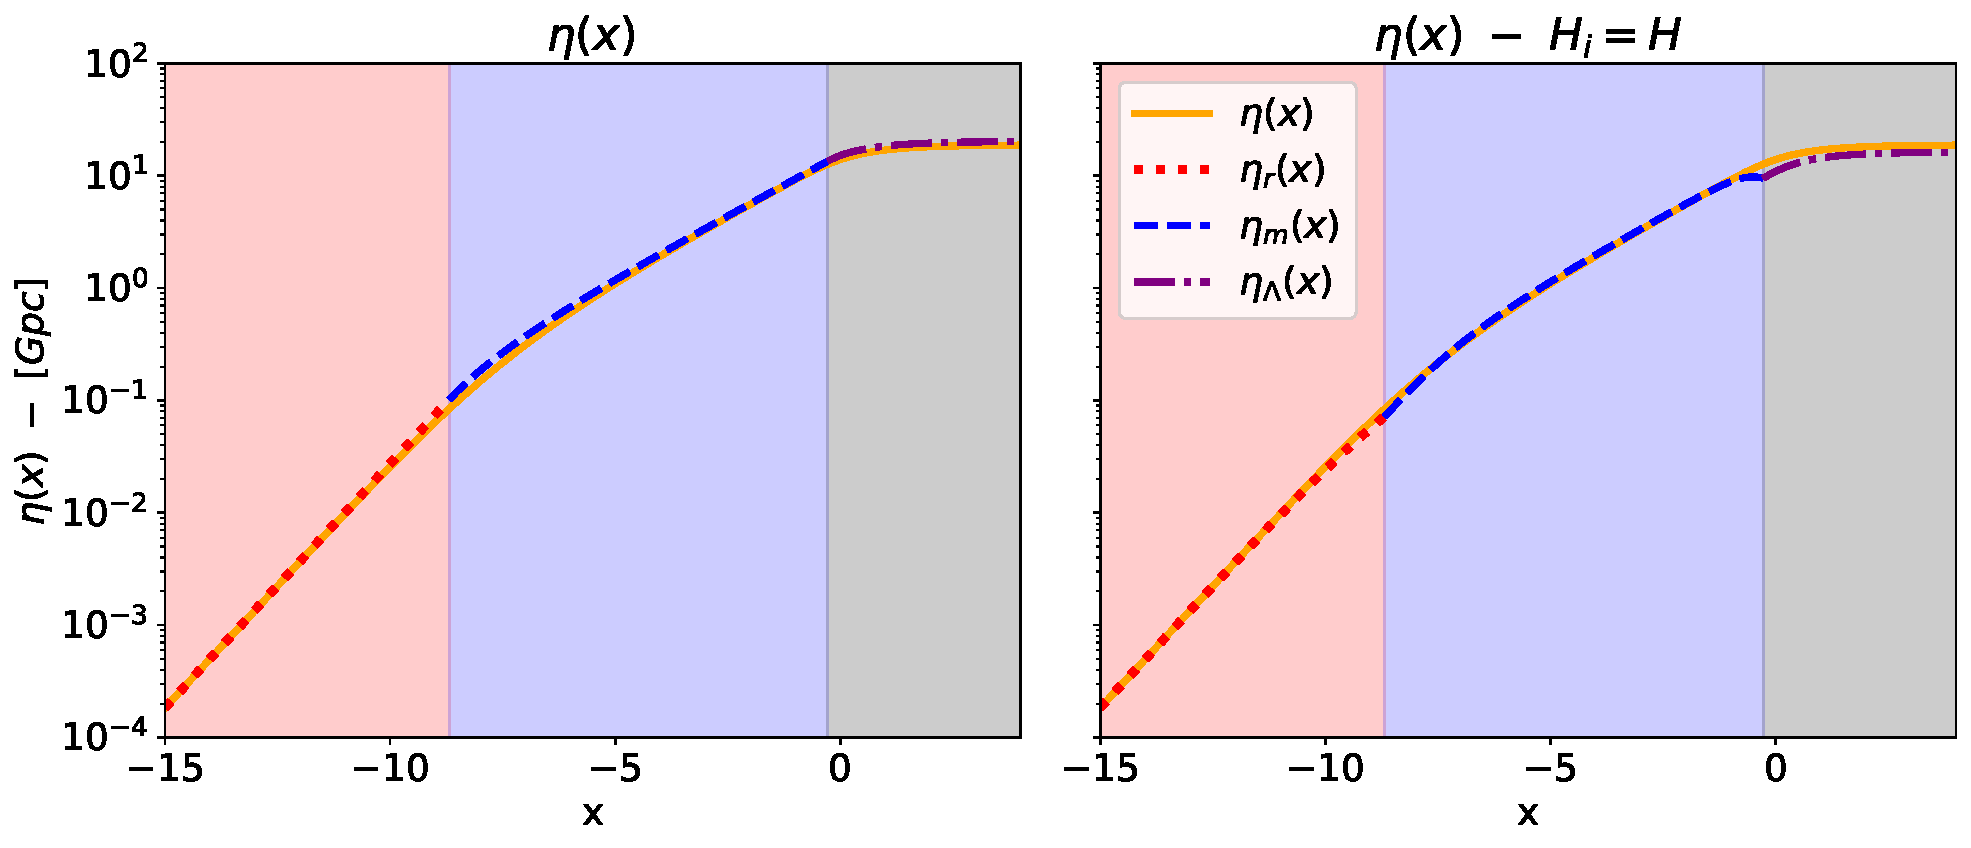
\includegraphics[scale=0.5]{../m1_figs/Eta2.pdf}
    \caption{Plot showing the three analytical approximations of $\eta(x)$ in the three regimes, together with the numerical solution (orange line). The "anchor" values of $a_*$ and $a_\Lambda$ are taken from the analytical approximation in the previous regime, making this a completely analytical expression. Left: The Hubble parameters are left as their local approximations. Right: The Hubble parameters are given their full expression, $H_i = H(x)$.}
    \label{fig:Eta2}
\end{figure}


\bibliography{ref}
\bibliographystyle{plain}



\end{document}